\section{O refinamento por realização}\label{sec:ref:metodo}

Cada realização do Monte Carlo do \texttt{SlopeRandomField} é calculada em três etapas: $\Gamma$ numa malha grossa, uma
malha refinada só em volta da banda de ruptura \emph{dessa} realização e $\Gamma$ de novo nela. Em vez de dividir
elementos dentro do NeoPZ, o gmsh gera uma malha conforme, sem nós pendurados; o NeoPZ só lê outro \texttt{.msh}. O C++
não muda: o executável é o do \texttt{SlopeRandomField}, e o projeto \texttt{SlopeRandomFieldRefina} tem só dois
scripts, \texttt{srf\_refinado.sh} (as três etapas) e \texttt{refina\_banda.py} (a etapa~2).

\subsection{As três etapas}\label{sec:ref:etapas}

\begin{enumerate}
\item \textbf{Malha grossa.} A realização roda na malha grossa \texttt{MALHA} (na comparação abaixo, a
  \texttt{foco375}, com elementos de 0,375~m na região das bandas), na pasta \texttt{grossa/}, gravando só os pontos
  de integração da banda (\texttt{mecanismo.csv}) e nenhum VTK.
\item \textbf{Malha refinada.} A banda são os pontos de integração com
  $\sqrt{J_2(\bm\varepsilon_p)} \ge 0{,}1\,\max \sqrt{J_2(\bm\varepsilon_p)}$ (\texttt{REFINA\_LIMIAR}), no último
  estado convergido da busca do fator, no instante do menor $\Gamma$ de \texttt{fs.csv}; é a mesma definição de banda do
  \texttt{BANDA\_LIMIAR} do programa. Os pontos são arredondados numa grade de $h = 0{,}125$~m (\texttt{REFINA\_H}):
  as \emph{células da banda}. O \texttt{.geo} novo é o da malha grossa (a mesma geometria, os mesmos grupos físicos e
  os mesmos campos de tamanho) com mais um campo de tamanho, função da distância $d$ às células da banda:
  \begin{equation}
    h_{\mathrm{b}}(d) =
    \begin{cases}
      h, & d \le f,\\[2pt]
      h + (h_{\max} - h)\,\dfrac{d - f}{3~\mathrm{m}}, & f < d < f + 3~\mathrm{m},\\[6pt]
      h_{\max}, & d \ge f + 3~\mathrm{m},
    \end{cases}
    \qquad
    h_{\mathrm{novo}}(\bm x) = \min\bigl(h_0(\bm x),\, h_{\mathrm{b}}(d(\bm x))\bigr),
    \label{eq:ref:campo}
  \end{equation}
  com a folga $f = 0{,}375$~m (\texttt{REFINA\_FOLGA}), $h_{\max}$ o tamanho máximo da malha grossa e $h_0$ o campo de
  tamanho dela (no gmsh, um campo \texttt{Distance}, um \texttt{Threshold} e um \texttt{Min} com o campo de fundo
  antigo). O gmsh gera a malha refinada, conforme; o NeoPZ a lê como qualquer outra malha.
\item \textbf{A mesma realização na malha refinada}, com os mesmos \texttt{REAL}, \texttt{CAMPOS} e \texttt{SEMENTE},
  na pasta da realização. As saídas são as do programa, e \texttt{resultado.txt} marca a realização como concluída.
\end{enumerate}
Sem banda na malha grossa (fator não positivo, ou o transiente não chegou ao instante do fator), não há onde refinar: o
resultado é o da malha grossa, marcado com \texttt{metodo=grossa} em \texttt{refino.csv}.

\paragraph{Por que o campo aleatório não muda.} O \texttt{SlopeRandomField} calcula os modos de Karhunen-Loève no
retângulo que contém os nós da malha e os avalia nas coordenadas dos pontos de integração; os números aleatórios de
cada campo ($c'$, $\varphi'$, $k$) vêm de \texttt{SEMENTE}, \texttt{REAL} e do campo. A malha refinada sai do mesmo
\texttt{.geo}, com o mesmo contorno; logo, o retângulo, os modos e os números aleatórios são os mesmos, e só mudam os
pontos onde o campo é avaliado: o campo é uma função das coordenadas, definida no retângulo, e a malha só escolhe onde
ela é avaliada. Conferido nas malhas refinadas do det e das realizações 0, 1, 3, 5 e 7 da comparação: a mesma caixa dos
nós (0 a 25~m por 0 a 10~m), os mesmos cantos, grupos físicos e elementos de contorno na base e nas laterais; nos pontos
de integração que coincidem nas duas malhas (de 6 a 21 por realização, longe da banda), os mesmos $c'$, $\varphi'$ e
$k$ nos 7 algarismos gravados; e, numa campanha do \texttt{rodar\_mc.sh}, \texttt{KL\_M} e \texttt{KL\_variancia}
iguais nas duas etapas. As médias de $c'$, $\varphi'$ e $k$ na área mudam entre as etapas em até 0,9\,\%, 0,3\,\% e
1,8\,\% nas realizações 0 a 7, porque os pontos de integração são outros (entre a \texttt{foco375} e a
\texttt{foco125}, em até 0,7\,\%, 0,4\,\% e 2,0\,\%), contra um desvio padrão de 13,5\,\%, 4,8\,\% e 19,6\,\% da
média de uma realização para outra.

\paragraph{Numa campanha.} O \texttt{srf\_refinado.sh} entra no lugar do executável no \texttt{rodar\_mc.sh}
(\texttt{EXE}), com \texttt{MALHA} a malha grossa (com o \texttt{.geo} ao lado); tudo o mais (variáveis do modelo,
\texttt{COMBS}, \texttt{PARALELO}, \texttt{SAIDA}, a junção e o resumo) é como no \texttt{SlopeRandomField}. A
retomada é por etapa: a~1 é pulada se há \texttt{grossa/resultado.txt}; a~2, se há \texttt{refino.csv} com os mesmos
\texttt{REFINA\_*} e o \texttt{.geo}; a~3 continua do \texttt{checkpoint.bin} do programa, como uma realização comum.
Um sinal termina o script com o código do sinal, e o \texttt{rodar\_mc.sh} o trata como trataria o programa (o Ctrl-C
não conta como falha; um \texttt{SIGKILL}, como o do OOM killer, conta). Depois do sucesso, \texttt{malha\_refinada.msh},
\texttt{grossa/mecanismo.csv} e um \texttt{checkpoint.bin} que tenha sobrado em \texttt{grossa/} são apagados; o
\texttt{.geo} (cerca de 20~kB) fica, e a malha é refeita dele se a realização for rodada de novo. Os \texttt{REFINA\_*}
de uma combinação ficam em \texttt{refino\_parametros.txt}, e outra rodada na mesma pasta com outros valores é
recusada. Cada realização tem um \texttt{refino.csv} com $\Gamma$ na malha grossa, as células da banda, os triângulos
da malha refinada, $\Gamma$ final e o tempo de cada etapa.

\subsection{Comparação com as malhas fixas}\label{sec:ref:comparacao}

O exemplo saturado do Ceron, com $\Gamma$ pelo GIM com arc-length em $t = 0{,}01$~h, em 9 casos (o determinístico,
\texttt{det}, com os parâmetros médios, e as realizações 0 a 7), cada um com cinco métodos:
\begin{itemize}
\item \texttt{foco375}, \texttt{foco25}, \texttt{foco1875} e \texttt{foco125}: o programa direto nas malhas
  \texttt{ceron\_h5\_a45\_foco*}, com elementos de 0,375, 0,25, 0,1875 e 0,125~m numa região fixa, a mesma nas quatro
  (as bandas do determinístico e das realizações 0 a 31 do exemplo, mais 0,75~m);
\item \texttt{refinada}: o \texttt{srf\_refinado.sh} com a malha grossa \texttt{foco375} e os padrões ($h = 0{,}125$~m,
  $f = 0{,}375$~m, limiar 0,1): em volta da banda, os elementos têm o tamanho dos da \texttt{foco125}.
\end{itemize}
A referência é a \texttt{foco125}, e a diferença de um método num caso é $\Gamma/\Gamma_{\mathrm{foco125}} - 1$. Os 45
casos rodaram numa fila só, com dois processos ao mesmo tempo (\texttt{PARALELO=2}), um thread por processo e o solver
skyline (máquina de 4 núcleos, sem MKL), intercalando os métodos caso a caso para que a carga da máquina, compartilhada
com outros trabalhos, pesasse sobre todos. O tempo de parede é o do processo inteiro (no método de duas malhas, as três
etapas e o gmsh); o de CPU é usuário + sistema do processo e dos descendentes. Como a carga variou, as tabelas trazem os
dois.
\IfFileExists{secoes/figs_malhas_comparacao.tex}{As malhas fixas estão na Fig.~\ref{fig:ref:malhas_fixas}; as etapas do
método, no determinístico, na Fig.~\ref{fig:ref:metodo_det}; e as malhas refinadas das realizações 0 a 7, na
Fig.~\ref{fig:ref:refinadas}.}{}

\IfFileExists{secoes/figs_malhas_comparacao.tex}{% figs_malhas_comparacao.tex: figuras de malhas da comparacao entre malhas fixas e refinamento pela banda.
% Gerado por figuras_malhas.py (python3 figuras_malhas.py comparacao); usa malhas.py.

\begin{figure}[htbp]
  \centering
  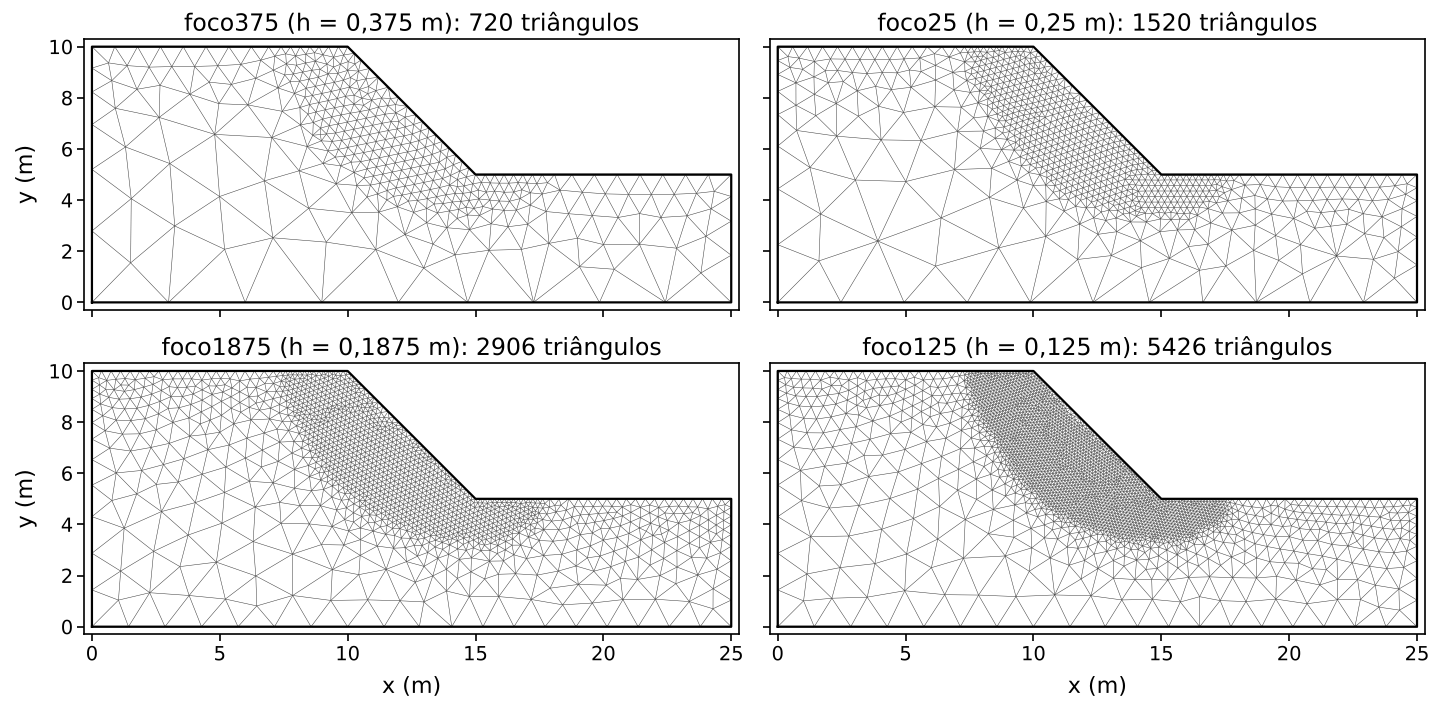
\includegraphics[width=\textwidth]{figuras/ref_malhas_fixas.png}
  \caption{Malhas fixas focadas da comparação (triângulos lineares, gmsh): tamanho $h$ de
    0,375, 0,25, 0,1875 e 0,125~m numa faixa de 0,75~m em torno das bandas de ruptura
    ($\sqrt{J_2} \geq 0{,}1$ do máximo) do caso determinístico e das realizações 0 a 31 de um
    estudo anterior na malha original; fora dela, 0,9~m perto da superfície e até 3~m no interior.
    Talude de Vargas Ceron et al.\ (2025), Seção~6: $H = 5$~m, $\beta = 45^\circ$, pé em (15, 5)
    e crista em (10, 10). A foco125 é a referência das diferenças relativas.}
  \label{fig:ref:malhas_fixas}
\end{figure}

\begin{figure}[htbp]
  \centering
  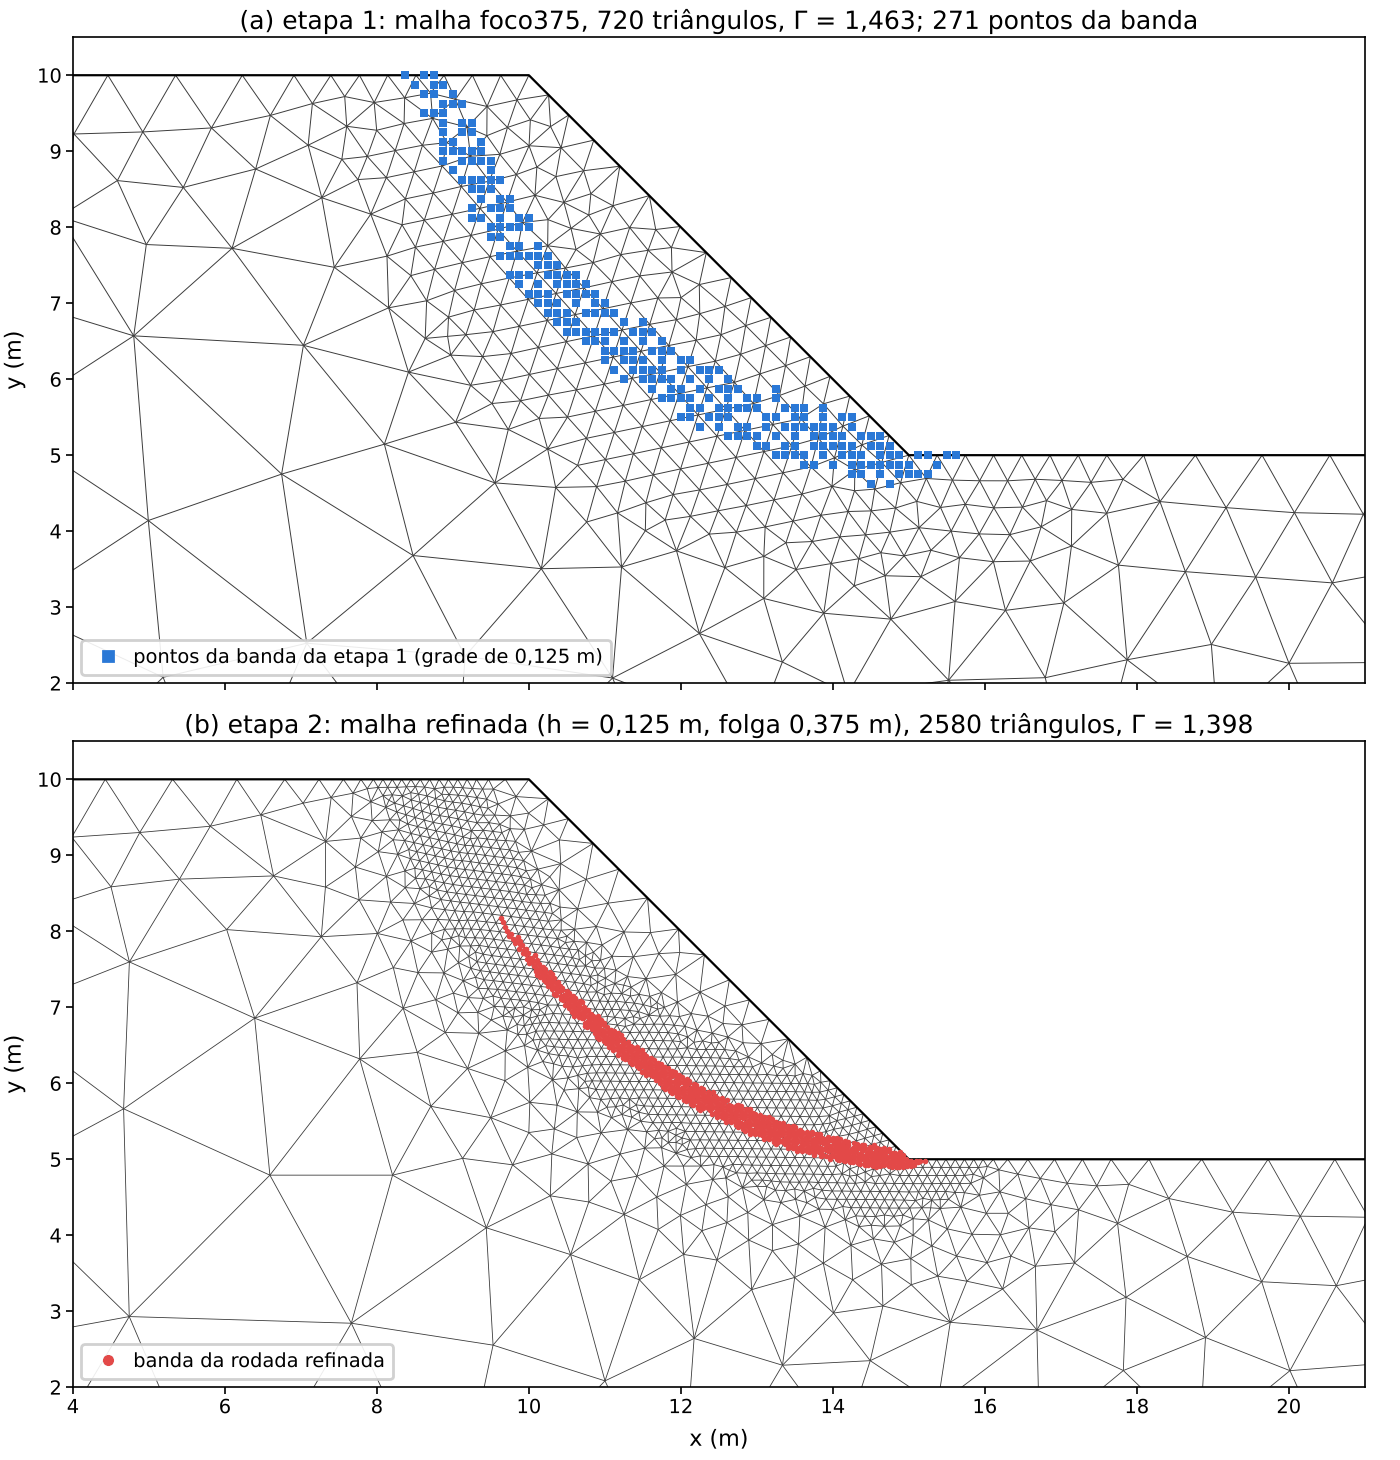
\includegraphics[width=\textwidth]{figuras/ref_metodo_det.png}
  \caption{Refinamento pela banda no caso determinístico (ampliação da região do talude).
    (a) Etapa~1: rodada na malha foco375 (720 triângulos, $\Gamma = 1{,}463$); os 271 pontos
    azuis são os pontos de integração da banda dessa rodada ($\sqrt{J_2}$ da deformação plástica
    $\geq 0{,}1$ do máximo no instante do fator, isto é, no $t_h$ do menor FS) arredondados numa
    grade de 0,125~m, que o \texttt{refina\_banda.py} acrescenta ao \texttt{.geo}.
    (b) Etapa~2: malha refinada com $h = 0{,}125$~m até 0,375~m desses pontos (2580 triângulos,
    contra 5426 da foco125) e, em vermelho, a banda da rodada refinada, com a mesma definição
    ($\Gamma = 1{,}398$).}
  \label{fig:ref:metodo_det}
\end{figure}

\begin{figure}[htbp]
  \centering
  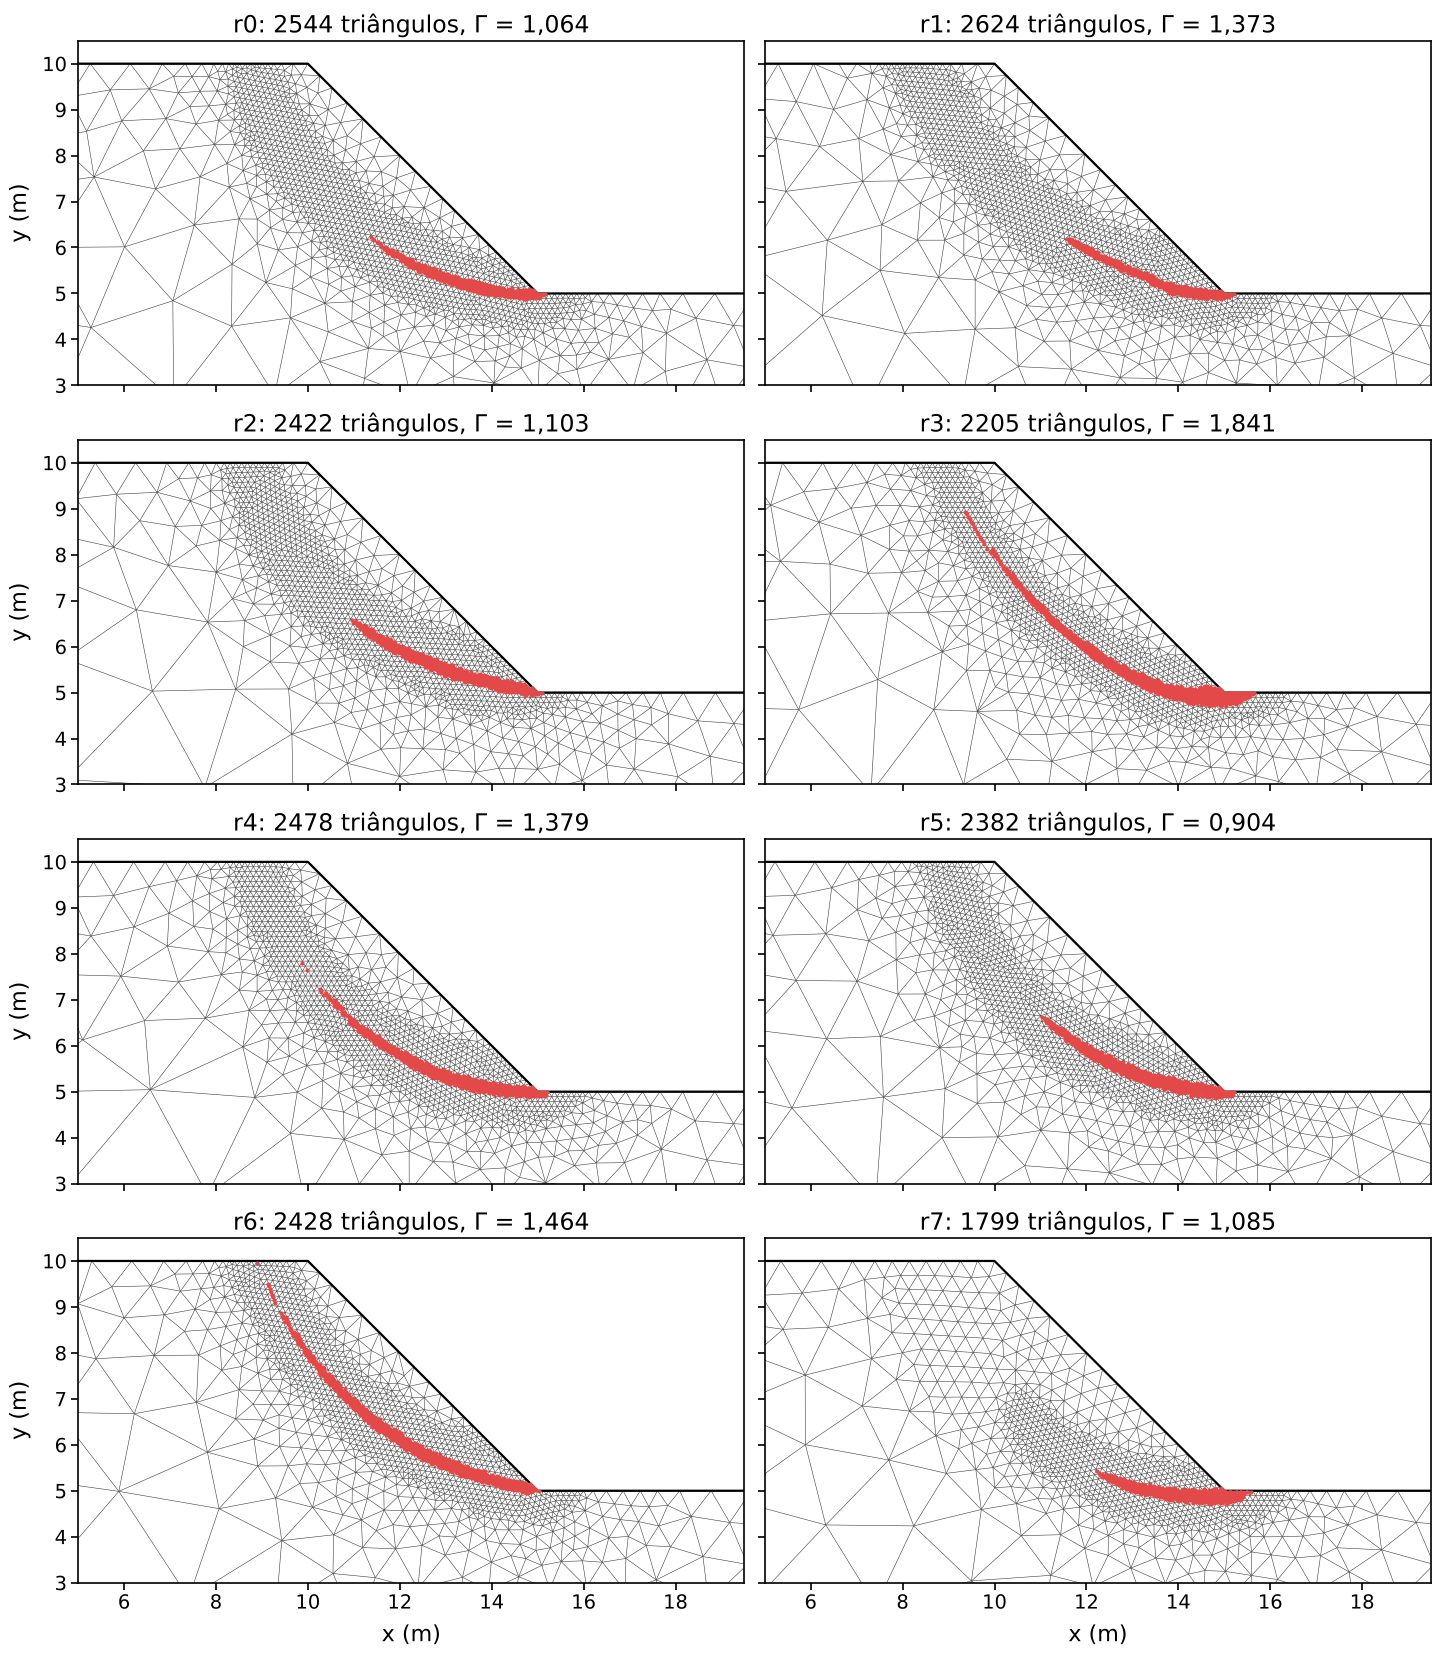
\includegraphics[width=\textwidth]{figuras/ref_refinadas.png}
  \caption{Malhas refinadas (etapa~2 a partir da foco375: $h = 0{,}125$~m até 0,375~m da banda da
    etapa~1) das realizações r0 a r7, com a banda de ruptura de cada rodada refinada (em vermelho:
    pontos de integração com $\sqrt{J_2}$ da deformação plástica $\geq 0{,}1$ do máximo no instante
    do fator) e o fator $\Gamma$ obtido. O número de triângulos acompanha a extensão da banda da
    etapa~1: de 1799 (r7, banda curta junto ao pé) a 2624 (r1), contra 5426 da malha fixa foco125.}
  \label{fig:ref:refinadas}
\end{figure}
}{}

\begin{table}[htbp]
  \centering\small\setlength{\tabcolsep}{3.5pt}
  \caption{Comparação por método, nos 9 casos (det e realizações 0 a 7): triângulos e equações (na \texttt{refinada},
    médias das malhas refinadas, de 1799 a 2624 triângulos), a diferença $\Gamma/\Gamma_{\mathrm{foco125}} - 1$ em valor
    absoluto (média e máximo) e com sinal (média), os tempos médios por caso e a razão deles para os da
    \texttt{foco125}. O tempo da \texttt{refinada} inclui a malha grossa e o gmsh.}
  \label{tab:ref:comparacao}
  % gerado por tabelas_comparacao.py a partir de dados/ref_comparacao.csv
\begin{tabular}{@{}lrrrrrrrrr@{}}
\toprule
 & & & \multicolumn{3}{c}{$\Gamma/\Gamma_{\mathrm{foco125}}-1$} & \multicolumn{2}{c}{tempo por caso (s)} & \multicolumn{2}{c}{razão p/ \texttt{foco125}} \\
\cmidrule(lr){4-6}\cmidrule(lr){7-8}\cmidrule(l){9-10}
método & triâng. & equações & $|\cdot|$ médio & $|\cdot|$ máx. & média c/ sinal & parede & CPU & parede & CPU \\
\midrule
\texttt{foco375} & 720 & 3808 & 5{,}17\,\% & 7{,}23\,\% & $+$5{,}17\,\% & 15{,}5 & 15{,}1 & 0{,}02 & 0{,}02 \\
\texttt{foco25} & 1520 & 7898 & 2{,}04\,\% & 3{,}21\,\% & $+$2{,}04\,\% & 57{,}5 & 53{,}3 & 0{,}09 & 0{,}09 \\
\texttt{foco1875} & 2906 & 14960 & 1{,}58\,\% & 2{,}24\,\% & $+$1{,}58\,\% & 184{,}5 & 179{,}7 & 0{,}29 & 0{,}29 \\
\texttt{refinada} & 2385 & 12199 & 0{,}23\,\% & 0{,}49\,\% & $+$0{,}14\,\% & 192{,}7 & 186{,}0 & 0{,}30 & 0{,}30 \\
\texttt{foco125} & 5426 & 27650 & --- & --- & --- & 634{,}4 & 616{,}7 & 1{,}00 & 1{,}00 \\
\bottomrule
\end{tabular}

\end{table}

\begin{table}[htbp]
  \centering\small\setlength{\tabcolsep}{4pt}
  \caption{$\Gamma$ de cada caso e método e, entre parênteses, a diferença para a \texttt{foco125}. r$i$ é a realização
    $i$.}
  \label{tab:ref:casos}
  % gerado por tabelas_comparacao.py a partir de dados/ref_comparacao.csv
\begin{tabular}{@{}lccccc@{}}
\toprule
caso & \texttt{foco375} & \texttt{foco25} & \texttt{foco1875} & \texttt{refinada} & \texttt{foco125} \\
\midrule
det & 1{,}4633 ($+$5{,}20\,\%) & 1{,}4210 ($+$2{,}15\,\%) & 1{,}4138 ($+$1{,}64\,\%) & 1{,}3976 ($+$0{,}47\,\%) & 1{,}3910 \\
r0 & 1{,}1224 ($+$5{,}22\,\%) & 1{,}0883 ($+$2{,}02\,\%) & 1{,}0845 ($+$1{,}66\,\%) & 1{,}0644 ($-$0{,}21\,\%) & 1{,}0667 \\
r1 & 1{,}4171 ($+$3{,}74\,\%) & 1{,}3889 ($+$1{,}67\,\%) & 1{,}3851 ($+$1{,}40\,\%) & 1{,}3727 ($+$0{,}49\,\%) & 1{,}3660 \\
r2 & 1{,}1731 ($+$6{,}15\,\%) & 1{,}1360 ($+$2{,}80\,\%) & 1{,}1298 ($+$2{,}24\,\%) & 1{,}1029 ($-$0{,}20\,\%) & 1{,}1051 \\
r3 & 1{,}9124 ($+$3{,}96\,\%) & 1{,}8688 ($+$1{,}59\,\%) & 1{,}8554 ($+$0{,}86\,\%) & 1{,}8413 ($+$0{,}09\,\%) & 1{,}8395 \\
r4 & 1{,}4702 ($+$6{,}79\,\%) & 1{,}4095 ($+$2{,}38\,\%) & 1{,}4036 ($+$1{,}95\,\%) & 1{,}3787 ($+$0{,}14\,\%) & 1{,}3767 \\
r5 & 0{,}9544 ($+$5{,}70\,\%) & 0{,}9216 ($+$2{,}06\,\%) & 0{,}9184 ($+$1{,}70\,\%) & 0{,}9037 ($+$0{,}08\,\%) & 0{,}9030 \\
r6 & 1{,}5654 ($+$7{,}23\,\%) & 1{,}5067 ($+$3{,}21\,\%) & 1{,}4897 ($+$2{,}04\,\%) & 1{,}4642 ($+$0{,}29\,\%) & 1{,}4599 \\
r7 & 1{,}1116 ($+$2{,}54\,\%) & 1{,}0896 ($+$0{,}51\,\%) & 1{,}0918 ($+$0{,}72\,\%) & 1{,}0852 ($+$0{,}11\,\%) & 1{,}0840 \\
\bottomrule
\end{tabular}

\end{table}

\paragraph{Precisão.} A \texttt{refinada} ficou a 0,23\,\% da \texttt{foco125} em média e a no máximo 0,49\,\%
(realização~1), dos dois lados (de $-0{,}21$\,\% a $+0{,}49$\,\%; Tabs.~\ref{tab:ref:comparacao}
e~\ref{tab:ref:casos}). As malhas fixas ficaram sempre acima da \texttt{foco125}: a \texttt{foco1875} a 1,58\,\% em
média (até 2,24\,\%), a \texttt{foco25} a 2,04\,\% (até 3,21\,\%) e a \texttt{foco375} a 5,17\,\% (até 7,23\,\%). O
$\Gamma$ da etapa~1 é o da \texttt{foco375} (os 9 valores são iguais): a etapa~3 leva a diferença de 5,17\,\% a
0,23\,\%. A realização~5 tem $\Gamma < 1$ nos cinco métodos, e as outras, $\Gamma > 1$ nos cinco. A banda final da
\texttt{refinada} ficou a no máximo 0,16~m das células da banda da malha grossa, dentro da região de elementos de
0,125~m, e nenhum caso ficou sem banda na malha grossa.

\paragraph{Tempo.} Com a malha grossa e o gmsh, a \texttt{refinada} levou 192,7~s de parede por caso (186,0~s de CPU):
30\,\% do tempo da \texttt{foco125} e 4\,\% mais que a \texttt{foco1875}, que fica a 1,58\,\%. Em média, a etapa~3 é
91,6\,\% do tempo de parede (176,4~s), a malha grossa 8,0\,\% (15,3~s) e o gmsh 0,3\,\% (0,64~s; de 0,16 a
0,20~s por malha, exceto 4,3~s na realização~0). A malha refinada teve
de 1799 a 2624 triângulos (de 9242 a 13412 equações), 18\,\% menos equações que a \texttt{foco1875} e 56\,\% menos que a
\texttt{foco125}; a busca do fator nela precisou de mais iterações de Newton (101,7 em média, contra 83,7 a 93,4 nas
malhas fixas). Repetidos o det e a realização~7 com os cinco métodos, os fatores foram os mesmos em todos os
algarismos, e os tempos de parede mudaram de $-6{,}7$\,\% a $+3{,}9$\,\%.

\paragraph{Ressalva: a \texttt{foco125} não está convergida.} A \texttt{refinada} e a \texttt{foco125} têm elementos de
0,125~m em volta da banda e ainda assim diferem em até 0,49\,\%: com elementos de 0,125~m, $\Gamma$ ainda depende da
malha nessa ordem de grandeza. As diferenças acima são, portanto, para a \texttt{foco125}, e não o erro em relação ao $\Gamma$ convergido. Nas
malhas fixas, $\Gamma$ cai quando os elementos diminuem (exceto entre a \texttt{foco25} e a \texttt{foco1875} na
realização~7), o que sugere um $\Gamma$ convergido abaixo do da \texttt{foco125}; a Seção~\ref{sec:ref:niveis} trata
dos níveis de refinamento.

\paragraph{Verificação independente.} Uma verificação independente recalculou as tabelas das saídas de cada caso,
conferiu os campos aleatórios nos pontos coincidentes, repetiu medições de tempo e rodou campanhas do
\texttt{rodar\_mc.sh} interrompidas em cada etapa (\texttt{kill -9}, \texttt{SIGINT}, \texttt{SIGKILL} só no programa),
além de um executável falso para os outros ramos do \texttt{srf\_refinado.sh}, e aprovou o método e os números. Os
defeitos encontrados foram corrigidos: a tolerância na comparação do instante da banda (7 algarismos em
\texttt{mecanismo.csv} e 10 em \texttt{fs.csv}; com passos como $\Delta t = 1/60$~h a banda ficaria vazia), o
\texttt{checkpoint.bin} que podia sobrar em \texttt{grossa/} depois de uma queda e trechos do README. Fica uma janela
de milissegundos: uma queda entre o programa da etapa~3 gravar \texttt{resultado.txt} e o script regravar
\texttt{refino.csv} deixa a realização concluída, com o $\Gamma$ da malha refinada, mas com o \texttt{refino.csv} sem as
colunas da etapa~3 e a malha e a banda ainda na pasta.
